\documentclass[]{article}
\usepackage[english]{babel}
\usepackage[explicit]{titlesec}
\usepackage{graphicx}

%opening
\title{Distributed Systems: Java RMI report}
\author{Tobias De Locht, Dries De Backker}
\date{3 November, 2017}

\begin{document}

\maketitle

\section{Design decisions}
The set up of this project consist of 2 packages, the client and the rental server. Figure \ref{fig:class} shows the class diagram of the project. For real life application a web server is needed so the client can download the necessary implementation classes. This deployment is visualized in figure \ref{fig:dep}.
\\
When starting up the rentalserver, it's main method creates a new namingService object. This object is mainly responsible for registering car rental companies and looking up their objects by name. The main method also creates a new remotely accessible sessionManager object. This object is in charge of creating new sessions for clients as well as managers. So two type of session classes are available with each it's corresponding remote interface class. Figure \ref{fig:client} shows a sequence diagram for a session creation by the client.
\\
The manager sessions are stateless while the reservation sessions are stateful. The reservation sessions are used by clients to check car availabilities and make or cancel reservations. The responsibilities of the manager is registering companies and obtaining statistics about the rental companies. The sequence diagram for making a reservation is shown in figure \ref{fig:reservation}.
\\
TODO: life cycle van de sessions?

 
\section{Remote objects}
There are 3 remote classes, each with there corresponding remote interface. The sessionManager, reservationSession and mangerSession classes.
TODO: welke objecten zijn remote en waarom? welke objecten moeten hierdoor serializable zijn? Welke objecten zijn geregistreerd in de RMI registry en waarom? welke remote objecten zijn gelocaliseerd op dezelfde host en waarom?
\section{Synchronization}
With the current deployment at use, it is possible multiple clients are concurrently sending method requests to the server. These request are then executed in interleaving threads. This way some data can become inconsisten.  To solve this problem some methods at the server are defined as synchronized. This will make it impossible for these methods to interleave their thread executions and execute sequential instead. The methods to made synchronized are in the carRentalCompany class and are the ones that can be requested directly by one of the sessions objects.
\clearpage
\section{Diagrams}
{\begin{figure}[h]
		\caption{Class Diagram}
		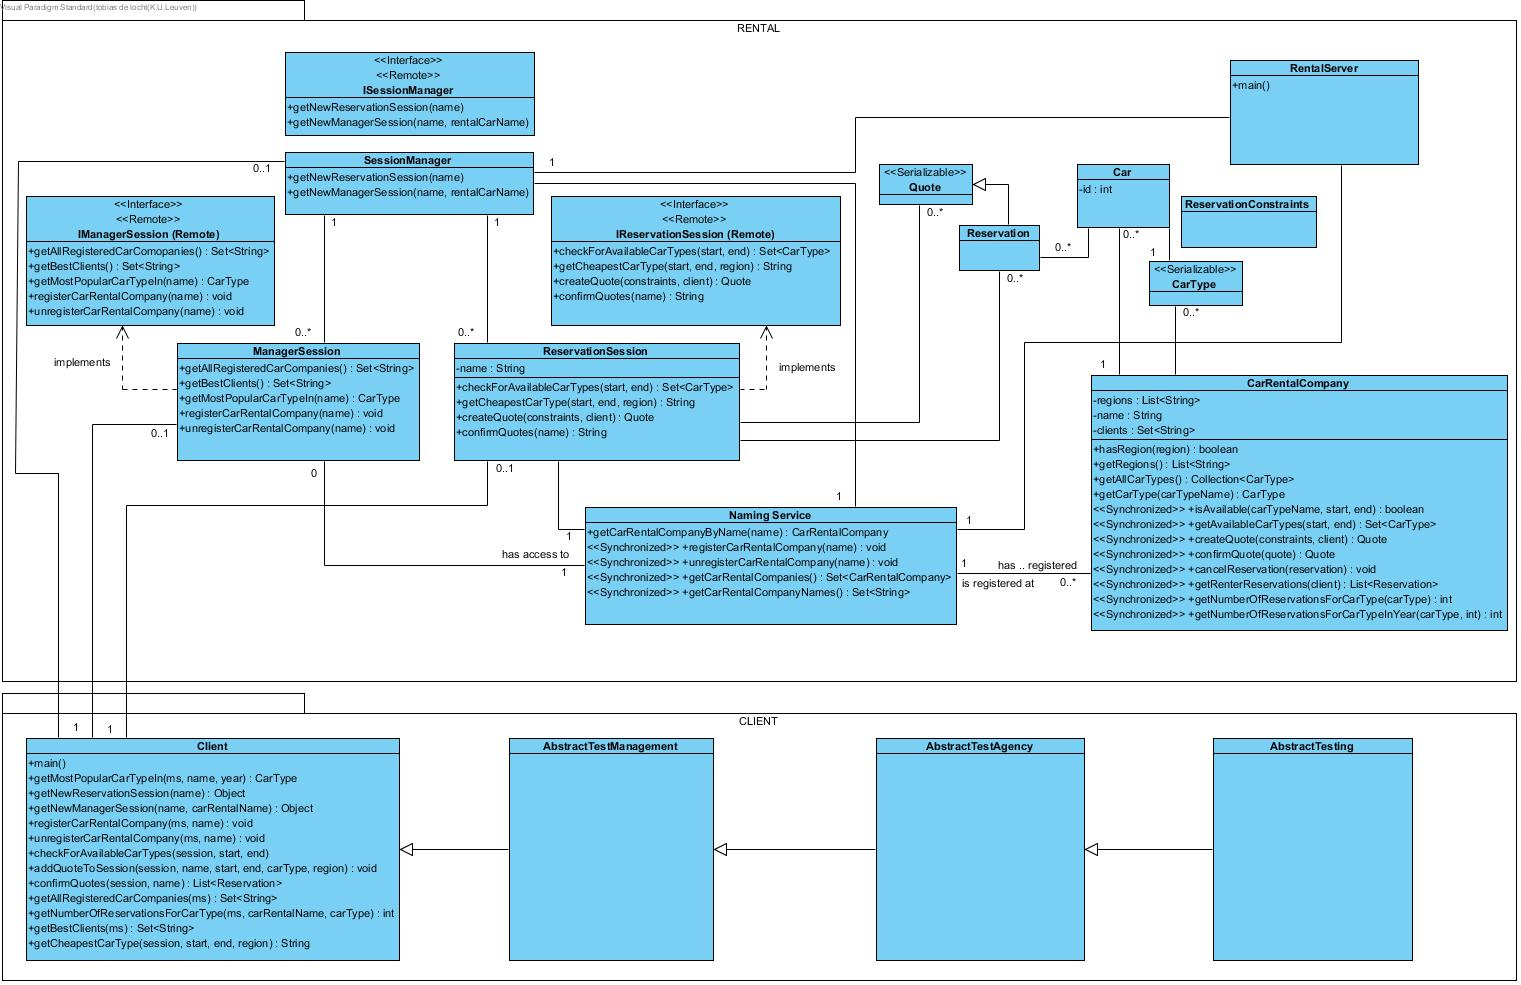
\includegraphics[width=1\textwidth]{classdiagram}
		\label{fig:class}
	\end{figure}
\clearpage
{\begin{figure}[h]
		\caption{Client session creation}
		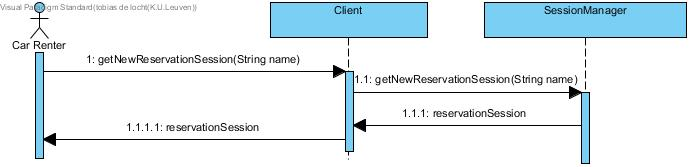
\includegraphics[width=1\textwidth]{clientseq}
		\label{fig:client}
	\end{figure}
{\begin{figure}[h]
		\caption{Reservation}
		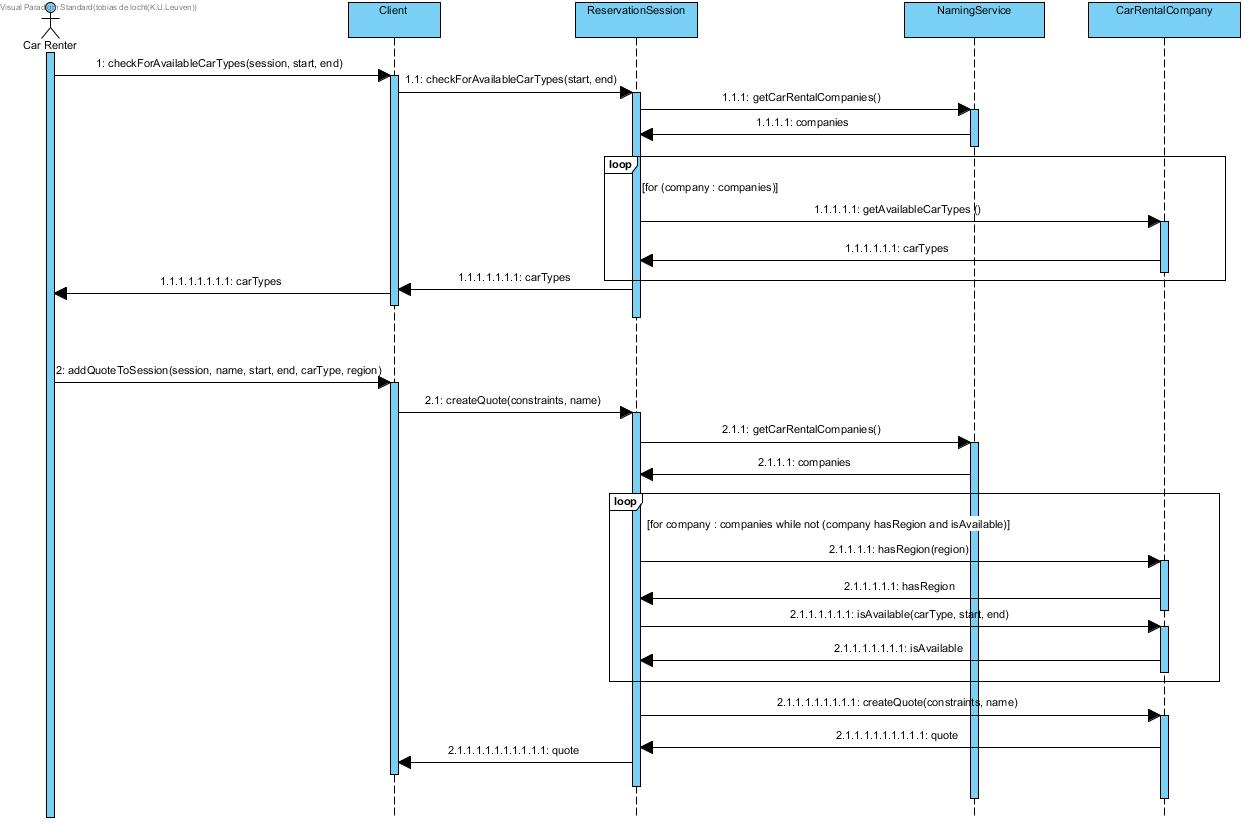
\includegraphics[width=1\textwidth]{reservationseq}
		\label{fig:reservation}
	\end{figure}
\clearpage
{\begin{figure}[h]
		\caption{Deployment}
		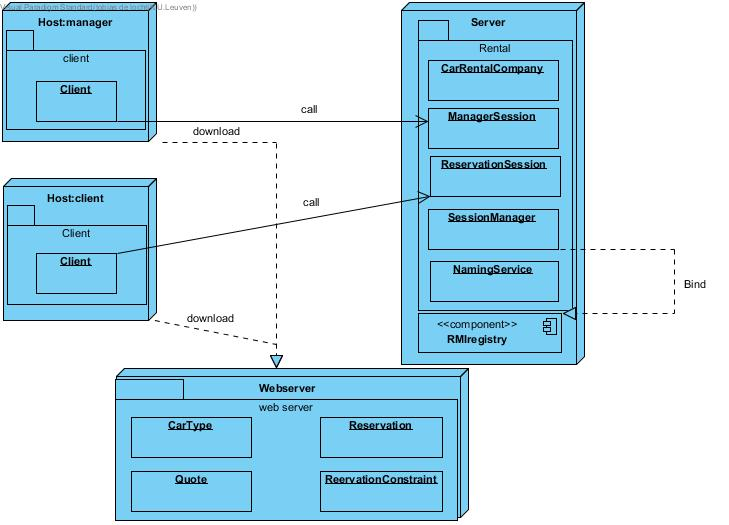
\includegraphics[width=1\textwidth]{deployment}
		\label{fig:dep}
	\end{figure}
\end{document}

